\documentclass[aspectratio=169,urlcolor=black]{beamer}
\usetheme[language=ngerman,
titlepagelogo=logopolito,
bullet=circle,
pageofpages=of,
color=blue,
titleline=true
]{TorinoTh}

%\usepackage[ngerman]{babel}
%\usepackage[utf8]{inputenc}
\usepackage{tabularx}
\usepackage{booktabs}
\usepackage{multicol}
\usepackage{ulem}
\usepackage{makecell}
\usepackage{upgreek}
\usepackage{movie15}
%\usepackage{xcolor}
%\usepackage{isodate}
\hypersetup{colorlinks,linkcolor=black,urlcolor=black}
\addto{\captionsngerman}{%
  \renewcommand*{\contentsname}{Contents}
  \renewcommand*{\listfigurename}{Figures}
  \renewcommand*{\listtablename}{Tables}
  \renewcommand*{\figurename}{Fig.}	
  \renewcommand*{\tablename}{Tab.}
}
\newcommand*\mean[1]{\bar{#1}}
\newcommand{\tabitem}{~~\llap{\textbullet}~~}
\newcommand\widebar[1]{\mathop{\overline{#1}}}
\usepackage{caption}
\captionsetup{font=scriptsize}

\usepackage{color}
\usepackage{graphicx}
\usepackage{fancybox}
\usepackage[singlespacing]{setspace}

\usepackage{beamerthemesplit}
\usetheme[compress]{Heidelberg}
\definecolor{unirot}{rgb}{0.4,0.4,0.3} % babyblue 0,0.58,1
\usecolortheme[named=unirot]{structure}
%\setbeamercolor{alerted text}{fg=red}
\newcommand*\hilite[1]{\textcolor{red}{#1}}
%\def\hilite<#1>{%
  %\temporal<#1>{\color{black}}{\color{unirot}}%
               %{\color{gray}}}

\title[Light Transport Techniques for Tensor Field Visualization]{Light Transport Techniques for Tensor Field Visualization}
\subtitle{Master's Thesis Presentation}
\vspace*{2pt}
\author[Sebastian Bek]{Sebastian Bek\vspace*{7pt}}
\date{July 24th 2019}
\institute[Uni HD]{
Heidelberg University\\
Visual Computing Group (VCG)\\
Supervisors: Prof. Filip Sadlo, Dr. Susanne Krömker\\
}

%\color{unirot}{sebibek@gmail.com}
%\newsubfloat{figure}
\newcommand{\source}[1]{\hspace{-3pt} {\tiny \raisebox{-0.75in}{\rotatebox[origin=t]{90}{Source: \color{black}{#1}}}}}
\setlength{\belowcaptionskip}{-10pt}
\setlength{\intextsep}{-20pt}

\setlength{\skip\footins}{0.1cm}
\setlength{\footnotesep}{0.1cm}
\renewcommand\thempfootnote{\arabic{mpfootnote}}
\begin{document}

%\frame[plain]{\titlepage}


\frame{
\frametitle{{Propagation Scheme - Template}}
\begin{columns}
\begin{column}{.6\textwidth}
To interpret eigensystems of tensors as conductivity property for light transport, we will need a propagation scheme:\bigskip
\begin{itemize}
	\item using light propagation volumes (LPV) similar to Dachsbacher et al. (cf. Fig.)\bigskip
	\item exchanging itensities between neighboring cells: $\Phi_{t} = \int I(\omega)\mathop{d\omega}$\\
	{\small with $\Phi_{t}$: radiant flux, $I(\omega)$: radiant intensity}
\end{itemize}

\end{column}
\begin{column}{.4\textwidth}
\begin{figure}[t]
\centering
\begin{minipage}{0.79\textwidth}
\centering
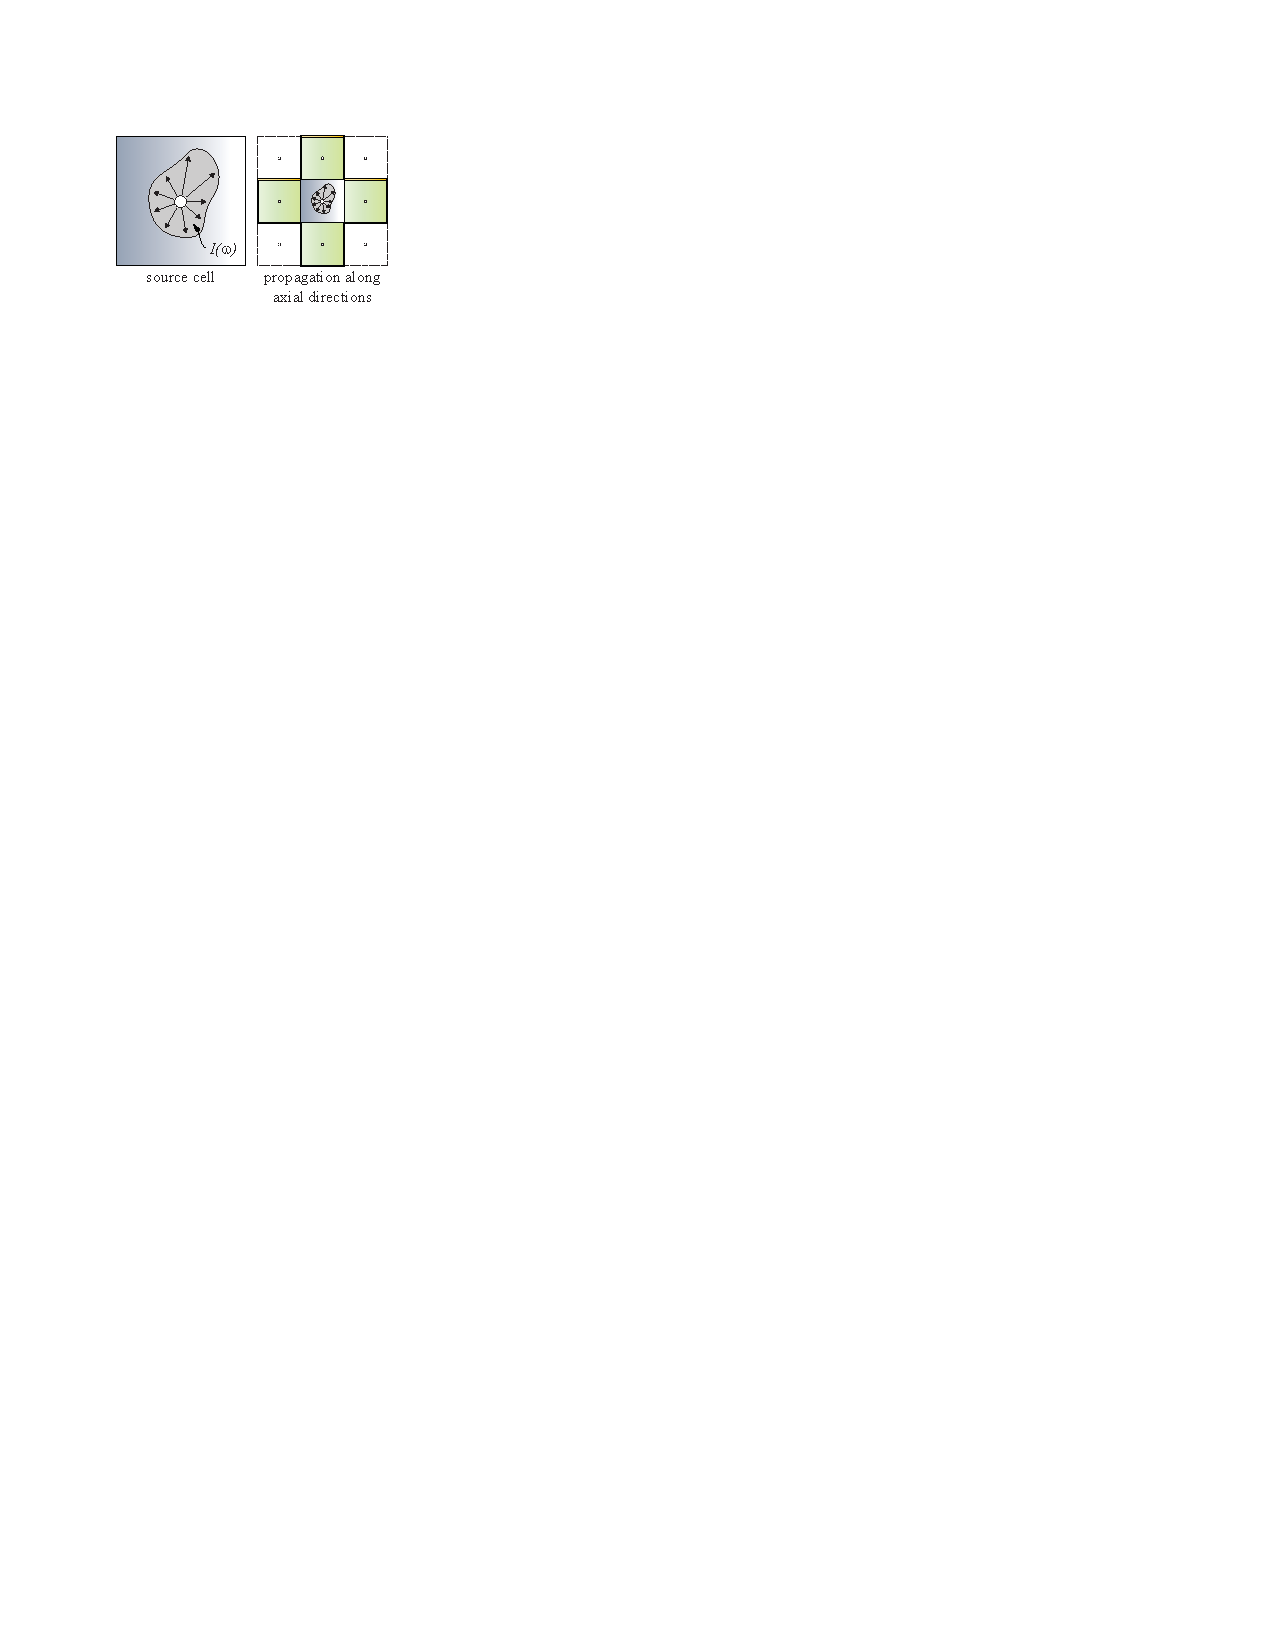
\includegraphics[width=0.7\textwidth]{LPV.pdf}
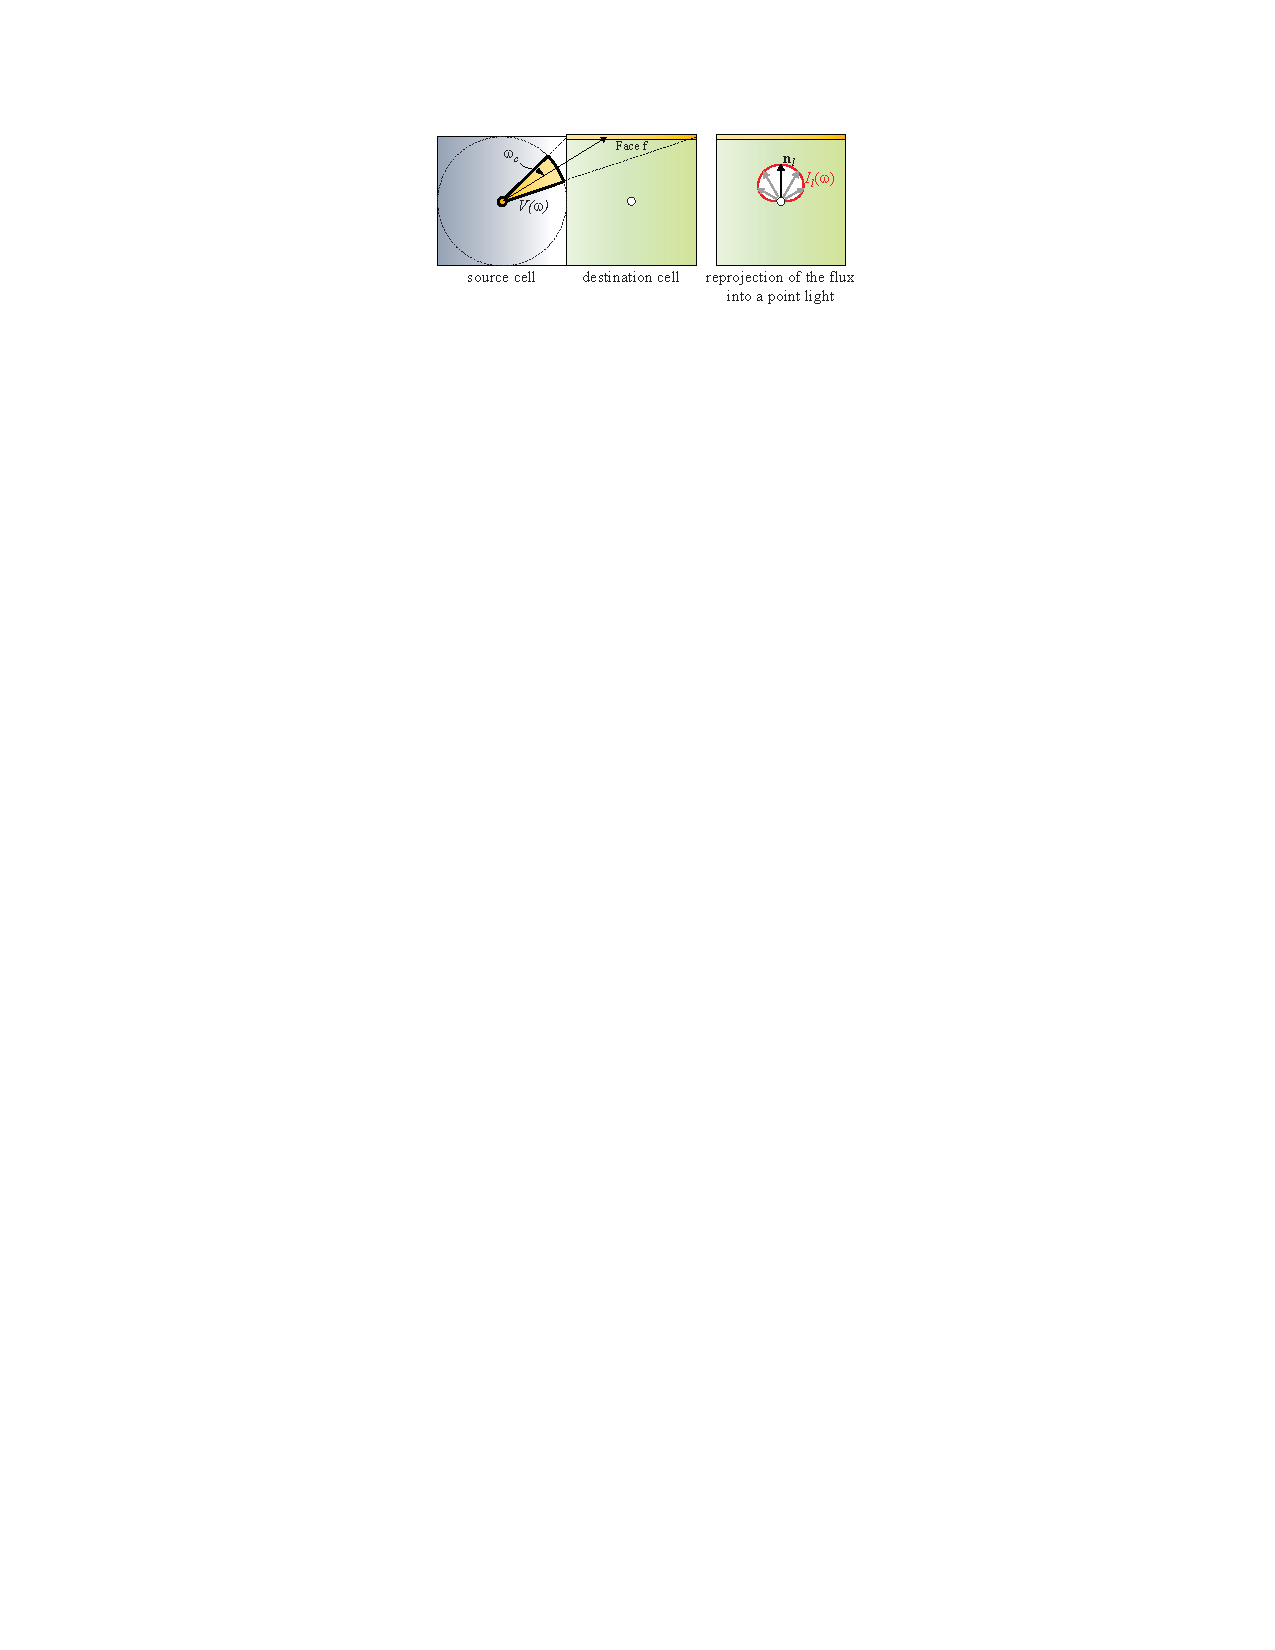
\includegraphics[width=0.9\textwidth]{LPV2.pdf}
\caption*{Light Propagation Volumes}
\end{minipage}
\begin{minipage}{0.15\textwidth}
\source{\textit{A. Kaplanyan and C. Dachsbacher, ''Cascaded light}} 
\hspace{-3pt} {\tiny \raisebox{-0.75in}{\rotatebox[origin=t]{90}{propagation volumes for realtime indirect illumination"}}}
\end{minipage}
\end{figure}

\end{column}
\end{columns}
} % END OF FRAME



%glyphs are used to represent the eigensystem, i.e., the anisotropy characteristics and/or tensor magnitude
%Volume non-directionally dependent


%%%%%%%%%%%%%%%%%%%%%%%%%%%%%%%%%%%%%%%%%%%%%%%%%%%%%%%%%%%%

% Alternative: put content in separate files
% Check the difference between including these files using \input{filename} and \include{filename} and see which one you like better
%\chapter{Einleitung}\label{intro}
%\input{introduction}
%
%\chapter{Voraussetzungen}\label{bg}
%\input{background}



\end{document}
